\chapter{Marco metodológico}
\label{capitulo2}
\lhead{Capítulo 2. \emph{Marco metodológico}}

En este capítulo se detalla la representación utilizada para los cromosomas, la función objetivo, las adaptaciones particulares que se hizo a cada algoritmo evolutivo usado en el experimento, el proceso de validación cruzada, la técnica de estratificación, se presenta los conjuntos de datos usados para el experimento y se explica el método de entonación utilizado para ajustar los algoritmos evolutivos.

\section{Representación del cromosoma}

Sea T el conjunto de instancias a reducir de tamaño \texttt{n}, la representación usada para modelar el problema de selección de prototipos es el de un mapa de bits de tamaño \texttt{n}, donde cada bit representa una instancia $t_i \in T$; si el valor del bit i es 1, entonces la instancia $t_i \in S$, donde S es el conjunto reducido; si el bit i es 0, $t_i \notin S$. En este sentido, el conjunto S representado por el mapa de bits M se define como en la ecuación (2.1). Además un ejemplo se presenta en \ref{representacion}. Cabe destacar que en los algoritmos evolutivos, los mapas de bits se conocen como cromosomas y cada bit como gen.

\begin{equation}
S = \left\{ t_i \in T \mid i = 1 \dots n \land m_i = 1 \land m_i \in M \right\}
\end{equation} 

\begin{figure}[]
\centering
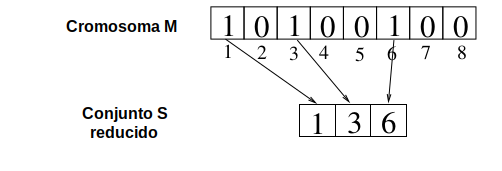
\includegraphics[height=3cm,width=10cm]{representacion.png}
\caption[Representación de un cromosoma y su respectivo conjunto reducido]{Representación de un cromosoma y su respectivo conjunto reducido}
\label{representacion}
\end{figure}

\section{Función objetivo}

Se necesita una función con la cual los algoritmos evolutivos puedan evaluar cuán buena es una solución dada, además de que dicha función debe permitir establecer una relación de orden entre las soluciones con el fin de decidir cuál cromosoma es mejor que otro. Como se explicó anteriormente, los algoritmos evolutivos buscan aproximarse al óptimo global, que en este caso es el conjunto reducido S con menor cardinalidad y mayor precisión en la clasificación de instancias nuevas. Es por eso que se adopta una función objetivo derivada del trabajo de \emph{Cano, J.} en \cite{de2004reduccion}, la cual se presenta a continuación:

\begin{equation}
\mathcal{F}(S) = \alpha * error(S) + (1 - \alpha) * reducción(S)
\end{equation} 

Donde $\mathcal{F}: S \rightarrow \mathbb{R}$ es la función objetivo, S es el conjunto reducido a evaluar, $\alpha$ es un parámetro que controla cuánta importancia se le da al error asociado a S con respecto a la tasa de reducción del segundo término de la ecuación (2.2), TR es el conjunto de entrenamiento original del cual se realizó la reducción, error(S) es el porcentaje de error al clasificar un conjunto de prueba TS usando 1-NN con S como conjunto de entrenamiento y reducción(S) es el porecentaje de instancias restantes en S en relación al conjunto original TR. El $\alpha$ usado es 0.5 como lo establecen en \cite{de2004reduccion} para darle la misma importancia a la reducción de datos como a mantener bajo los porcentajes de error en la clasificación.

Dado esta función objetivo, la meta de todas las metaheurísticas implementadas se vuelve minimizar $\mathcal{F}(S)$, lo cual quiere decir que se busca tanto reducir $\mid S \mid$, como reducir error(S). Una conjunto $S_i$ es mejor que un conjunto $S_j$ si $\mathcal{F}(S_i) < \mathcal{F}(S_j)$.  

\section{Adaptaciones de los algoritmos evolutivos}

Para aplicar los distintos algoritmos evolutivos implementados para este trabajo, es necesario determinar los operadores de cruce, mutación, el método de selección de los cromosomas que van a cruzarse, el criterio de selección de los cromosomas sobrevivientes y en caso del algoritmo memético el proceso de optimización interno (también conocido como meme) utilizado.

Para el caso del algoritmo genético estacionario y el algoritmo memético, se eligió como método se selección de cromosomas a cruzarse un proceso de torneo \cite{talbi2009metaheuristics}, el cual consiste en seleccionar k cromosomas de manera aleatoria y elegir el mejor de los k. CHC por su parte elige dos cromosomas aleatorios y utiliza su mecanismo de prevención de incesto para elegir a los padres. El algoritmo genético generacional simplemente elige dos elementos aleatorios para realizar el cruce.

El operador de cruce utilizado en GGA, SSGA y MA es el cruce de un punto \cite{talbi2009metaheuristics}, el cual consiste en definir un punto $\mu$ en el cual se va dividir los dos cromosomas seleccionados como padres y luego se forman dos hijos a partir de la mezcla de las partes de los padres. CHC en cambio usa el operador HUX explicado anteriormente. En la figura \ref{cruce} se muestra un ejemplo del cruce de un punto. 

\begin{figure}[]
\centering
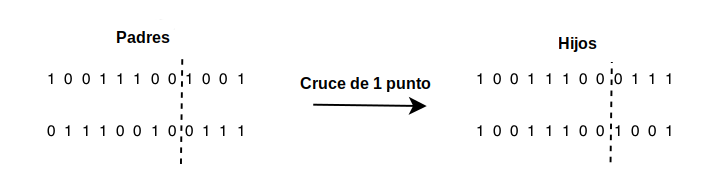
\includegraphics[width=\textwidth]{cruce.png}
\caption[Cruce de un punto]{Cruce de un punto}
\label{cruce}
\end{figure}

El operador de mutación para GGA, SSGA y MA consta de cambiar 5\% de los genes del cromosoma de manera aleatoria. Se elige 5\%  basado en \cite{flores2014metaheuristics} para que la mutación represente una variación en S, ya que si sólo se cambia un gen, el conjunto mutado sería para los efectos de la optimización casi idéntico al original. Sin embargo la probabilidad de que un cromosoma dado mute es baja, basado principalmente en los resultados de \emph{Cano, J.} en \cite{de2004reduccion} donde obtienen mejores resultados experimentales con bajas probabilidades de mutación (menor al 1\% por cromosoma), justificándose en que con mayores valores, la búsqueda podría degenerar en una búsqueda aleatoria. CHC por su parte no tiene mutación.

El criterio de reemplazo para GGA es generar una población nueva de hijos $P_i$ que va a suplantar la generación anterior $P_{i-1}$ excepto el mejor elemento en $P_{i-1}$. Por su parte, el criterio de reemplazo de SSGA es que dado dos padres y los dos hijos producidos por el operador de cruce, se eligen los 2 mejores cromosomas para permanecer dentro de la población. MA, en cambio usa un criterio de reemplazo en el cual los 2 hijos suplantan a los 2 peores elementos de la población y CHC se queda con los \texttt{n} mejores cromosomas entre $P_i$ y $P_{i-1}$, ambos casos son totalmente elitistas.

El algoritmo memético es el que más adaptaciones tiene para adecuarse a PS, se usa una adaptación realizado por \emph{Cano, J. et al.} en \cite{garcia2008memetic}. Se basa en el algoritmo memético estacionario presentado anteriormente, con la peculiariadad de que para decidir si los hijos producidos en una iteración van a ser optimizados con el meme, se usa un parámetro $P_{LS}$ que se determina de la siguiente forma:

\begin{equation}
P_{LS}=
\begin{cases}
1 & \text{si } \mathcal{F}(S_{nuevo}) < \mathcal{F}(S_{peor})\\
0.0625 & \text{en caso contrario}\\
\end{cases}
\end{equation}

Donde $\mathcal{F}$ es la función objetivo, $S_{nuevo}$ es el conjunto reducido representado por uno de los cromosomas hijos y $S_{peor}$ es el conjunto reducido representado por el peor cromosoma de la población. Es así como $P_{LS}$ representa la probabilidad con la cual se va a decidir si se optimiza el cromosoma hijo; $P_{LS}$ debe ser calculado para cada hijo creado en el cruce. La idea es que si el hijo es mejor que el peor cromosoma de la población, entonces vale la pena optimizarlo; en cambio, si es peor, se le da una probabilidad de optimización de 6,25\%.

El meme usado en MA es el que se presenta en el algoritmo \ref{meme}. El procedimiento consiste en ir reduciendo progresivamente las instancias que se encuentran en el conjunto S, representado por el cromosoma M, sin que se pierda la precisión asociada a S. Para esto, se usa una lista U del primer vecino más cercano de cada gen en M, una lista R que contiene los genes que ya han sido puestos en 0 y que no generan una ganancia mayor al umbral de aceptación \texttt{t}, clase(i) es la clase asociada a la instancia representada por el gen i del cromosoma M, \texttt{ganancia} representa cuánto mejora (en caso de que sea positiva) o cuánto empeora (en caso de ser negativa) la solución dada por el cromosoma M luego de cambiar un gen, $fitness_M$ es el valor de evaluar la función objetivo con el cromosoma M y $fitness_{ganancia}$ se define como en la ecuación (2.4), donde L es el largo del cromosoma:

\begin{equation}
fitness_{ganancia} = \frac{\frac{ganancia}{L}*100 + \frac{100}{L}}{2}
\end{equation}  

El meme intenta remover una instancia de S en cada iteración pra ver si la precisión mejora, se mantiene igual o empeora. Si la ganancia es positiva y está por encima del umbral de aceptación entonces se preservan los cambios; en cambio, si la ganancia está por debajo del umbral, entonces se vuelve a incluir la instancia eliminada y se etiqueta su respectivo gen como revisado.
 
\begin{algorithm}
\caption{Meme}
\label{meme}
\begin{algorithmic}[1]

\Require{\texttt{M} cromosoma a optimizar, \texttt{t} umbral de aceptación}
\Ensure{\texttt{M} cromosoma optimizado}

\State Sea $\texttt{M} = \left\{ m_1,m_2,\dots,m_n \right\}$ el cromosoma a optimizar 
\State $R \gets \emptyset$
\State $ U = \left\{ u_1,u_2,\dots,u_n \right\}$ la lista de vecinos asociados, donde $u_i$ es el vecino más cercano del gen i. 
\While{$(\exists m_i \in \texttt{M} \mid m_i = 1 \land i \notin R)$}
	\State elegir j aleatoriamente de \texttt{M} tal que $m_j=1 \land j \notin R$
	\State $ganancia \gets 0$
	\State $m_j \gets 0$
	\State Copiar U a U'
	\ForAll{$u_i \in U \mid u_i = j$}
		\State $u_i \gets$ nuevo vecino más cercano con el nuevo \texttt{M}
		\If{$clase(i) = clase(u'_i) \land clase(i) \neq clase(u_i)$}
			\State $ganancia \gets ganancia - 1$
		\ElsIf{$clase(i) \neq clase(u'_i) \land clase(i) = clase(u_i)$}
			\State $ganancia \gets ganancia + 1$
		\EndIf
	\EndFor
	\If{$ganancia \geq \texttt{t}$}
		\State \emph{$fitness_M$} $\gets$ \emph{$fitness_M$} + \emph{$fitness_{ganancia}$}
		\State $R \gets \emptyset$
	\Else
		\State Recuperar U de U'
		\State $m_j \gets 1$
		\State $ R \gets R \cup j$
	\EndIf
\EndWhile

\State \Return M

\end{algorithmic}
\end{algorithm}

\section{Criterios para comparar los métodos de selección de prototipos}

Al momento de comparar los distintos métodos de PS, se usan los siguiente criterios para evaluar las fortalezas y debilidades relativas de cada algoritmo \cite{garcia2016data}:

\begin{itemize}
\item \textbf{Reducción: }
se mide como la proporción existente entre la cardinalidad del conjunto reducido S entre el conjunto de entrenamiento; esto es $|S|/TR$. La reducción de las instancias trae consigo una disminución en los tiempos de cómputo al tener que revisar menos cromosomas en cada iteración para clasificar una nueva instancia. 

\item \textbf{Precisión de la clasificación: }
se espera que aún con el conjunto reducido, se mantenga las tasas de acierto del clasificador o inclusive, mejoren. Un algoritmo de PS debe poder mantener la precisión al momento de ser evaluado con el conjunto de prueba. La precisión se calcula dividiendo el número de clasificaciones hechas correctamente entre el total de clasificaciones.

\item \textbf{Tiempo de cómputo: }
involucra cuánto tiempo le lleva al algoritmo realizar la reducción de los datos, un factor importante al momento de escalar los métodos a conjuntos muy grandes. En este trabajo el tiempo de cómputo se mide en segundos.

\item \textbf{\emph{Cohen's Kappa}: } 
es una métrica que originalmente mide el nivel de acuerdo o desacuerdo entre dos clasificadores. Sin embargo se han hecho adaptaciones de esta métrica para ser usada por un sólo clasificador \cite{garcia2012prototype}, ya que es más robusta que la precisión por tomar en cuenta la posibilidad de que una clasificación sea hecha aleatoriamente. Esta métrica sirve para verificar si el clasificador está etiquetando las instancias correctamente de manera consistente o de una manera inestable con muchas decisiones aleatorias. \emph{Cohen's kappa} se calcula a partir de la matriz de confusión como se muestra en la ecuación (1.1). Donde $y_{ii}$ es el conteo de las celdas de la diagonal principal, N el número de instancias revisadas, $\Omega$ el el número de clases presentes, $y_i.$ es la suma de las celdas de la fila i y $Y._i$ es la suma de las celdas de la columna i.

\begin{equation} 
kappa = \frac{N*\sum_{i=1}^{\Omega}y_{ii} - \sum_{i=1}^{\Omega}y_i.*y._i}{N^2 - \sum_{i=1}^{\Omega}y_i.*y._i}
\end{equation}

\end{itemize}


\section{Conjunto de datos}

Los conjuntos de datos utilizados para validar el experimento provienen de \emph{UCI Machine Learning Repository} \cite{Dua:2017} y \emph{KEEL Data-Mining Software Tool} \cite{alcala2011keel}. Se hace una separación como la establecida en \cite{de2004reduccion} donde se considera como conjunto de datos pequeños aquellos con menos de 2000 instancias, los conjuntos medianos los que poseen entre 2000 y 20000 instancias y los conjuntos grandes aquellos con más de 20000 instancias. En la tabla \ref{pequenios} se detallan los conjuntos pequeños, en \ref{medianos} los medianos y en \ref{grandes} los grandes. Solo se eligió conjunto de datos numéricos para poder utilizar la distancia euclídea con 1-NN sin tener problemas en la preservación de información al convertir datos categóricos a numéricos.

\begin{table}[]
\centering
\begin{tabular}{l c c c}
\hline
\textsc{Conjunto} & \textsc{Instancias} & \textsc{Atributos} & \textsc{Clases} \\
\hline
\hline

Iris          & 150  &  4 &  3 \\
Cleveland     & 297  & 13 &  5 \\
Led7Digit     & 500  &  7 & 10 \\
Pima          & 768  &  8 &  2 \\
WDBC          & 569  & 30 &  2 \\
Monk-2        & 432  &  6 &  2 \\
Wisconsin     & 683  &  9 &  2 \\
Wine          & 178  & 13 &  3 \\
Glass         & 214  &  9 &  7 \\
Banknote      & 1372 &  5 &  2 \\
Appendicitis  & 106  &  7 &  2 \\
Balance       & 625  &  4 &  3 \\
Bands         & 539  & 19 &  2 \\
Contraceptive & 1473 & 9  &  3 \\
Dermatology   &  366 & 34 &  6 \\
Ecoli         &  336 &  7 &  8 \\
Haberman      &  306 & 3  &  2 \\
Hayes-roth    &  160 & 4  &  3 \\
Heart         &  270 & 13 &  2 \\
Hepatitis     &  155 & 19 &  2 \\
Mammographic  &  961 & 5  &  2 \\
Newthyroid    &  215 & 5  &  3 \\
Tae           &  151 & 5  &  3 \\
Vehicle       &  846 & 18 &  4 \\
Vowel         &  990 & 13 & 11 \\
Yeast         & 1484 & 8  & 10 \\
 
\hline
\end{tabular}
\caption{Conjuntos de datos pequeños}
\label{pequenios}
\end{table}

\begin{table}[]
\centering
\begin{tabular}{l c c c}
\hline
\textsc{Conjunto} & \textsc{Instancias} & \textsc{Atributos} & \textsc{Clases} \\
\hline
\hline

Banana           &  5300 &  2 & 2 \\
Cardiotocography &  2126 & 23 & 3 \\
Eye-state        & 14980 & 15 & 2 \\
Page-blocks      &  5473 & 10 & 5 \\
Penbased         & 10992 & 16 & 10 \\
Satimage         &  6435 & 36 & 7 \\
Thyroid          &  7200 & 21 & 3 \\
Segment          &  2310 & 19 & 7 \\
Coil2000         &  9822 & 85 & 2 \\
Magic            & 19020 & 10 & 2 \\
Marketing        &  8993 & 13 & 9 \\
Phoneme          &  5404 & 5  & 5 \\
Ring             &  7400 & 20 & 2 \\
Spambase         &  4597 & 57 & 2 \\
Texture          &  5500 & 40 & 11 \\
Titanic          &  2201 &  3 & 2  \\
Twonorm          &  7400 & 20 & 2 \\

\hline
\end{tabular}
\caption{Conjuntos de datos medianos}
\label{medianos}
\end{table}

\begin{table}[]
\centering
\begin{tabular}{l c c c}
\hline
\textsc{Conjunto} & \textsc{Instancias} & \textsc{Atributos} & \textsc{Clases} \\
\hline
\hline

Credit-card      & 30000 & 24 & 2 \\
Shuttle          & 58000 & 9  & 7 \\

\hline
\end{tabular}
\caption{Conjuntos de datos grandes}
\label{grandes}
\end{table}

\section{Validación cruzada y estratificación}

Dado un conjunto de datos T, el proceso de validación cruzada \cite{kohavi1995study} consta de dividir T en k subconjuntos disjuntos $T_1,T_2,\dots,T_k$ de aproximadamente el mismo tamaño, donde cada subconjunto mantiene la distribución de las clases presente en T. Luego se procede a probar el clasificador M, que en este caso es 1-NN, k veces, donde en cada prueba $t \in \left\{1,2,\dots,k\right\}$ se utiliza como conjunto de entrenamiento $TR=T \setminus T_t$, se aplica el algoritmo de selección de prototipos a TR y el conjunto resultante S se valida usando $TS=T_t$ como conjunto de prueba. El porcentaje de aciertos del clasificador se calcula como el promedio de las k pruebas realizadas; pero como las metaheurísticas tienen un componente estocástico, se necesita repetir cada prueba varias veces.  En la figura \ref{crossval} se muestra un esquema de cómo se aplica la validación cruzada para el problema de selección de prototipos dado que la partición k es seleccionada como conjunto de prueba.

\begin{figure}[]
\centering
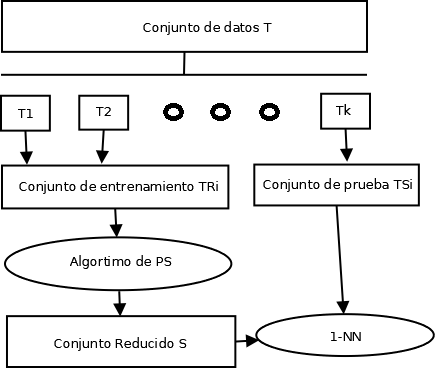
\includegraphics[scale=0.3]{classicCV.png}
\caption[Validación cruzada]{Validación cruzada}
\label{crossval}
\end{figure}

Por otra parte está la estratificación, la cual es una técnica propuesta por \emph{Cano, J. et al.} en \cite{cano2005stratification} para solventar el problema de aplicación de los algoritmos de PS a conjunto de datos muy grandes. Dicho problema viene dado porque la mayoría de los algoritmos de PS y metaheurísticas utilizadas son $O(n^2)$, siendo $n$ la cantidad de instancias del conjunto a procesar, y por lo tanto, para grandes volúmenes de datos estos algoritmos empiezan a tardar mucho en calcular una solución, lo cual los vuelve poco útiles al momento de hacer preprocesamiento de datos. Es así que la estratificación se adopta como una técnica que lleva a tiempos aceptables el cómputo con conjuntos de muchas instancias. 

Dado un conjunto de datos TR producto de la división hecha por un proceso de validación cruzada, la estratificación empieza dividiendo TR en k subconjuntos disjuntos, llamados estratos, $TR_1,TR_2,\dots,TR_k$ de aproximadamente el mismo tamaño. Luego, se aplica el algoritmo de PS directamente a cada uno de los $k$ subconjuntos seleccionados $TR_i$ para el entrenamiento, formando entonces subconjuntos reducidos $TRS_1,TRS_2,\dots,TRS_k$; acto seguido, se juntan todos los $TRS_i$ para formar el conjunto reducido S que va a ser usado por 1-NN para clasificar $TS$. La estratificación prueba ser un método efectivo, como lo demuestran en \cite{cano2005stratification}, ya que reduce la cantidad de instancias que debe tratar el algoritmo de PS a $TR/k$, por lo que la elección del número de estratos k se vuelve de especial importancia. En la figura \ref{strat} se muestra un esquema de cómo se aplica la estratificación, donde el estrato k es seleccionado como conjunto de prueba.

\begin{figure}[]
\centering
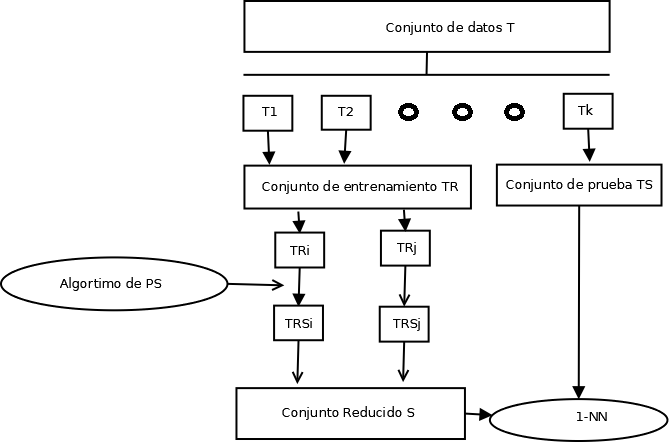
\includegraphics[scale=0.3]{stratCV.png}
\caption[Estratificación]{Estratificación}
\label{strat}
\end{figure}

\section{Entonación de las metaheurísticas}

Para la entonación de las metaheurísticas se usó \emph{irace} \cite{lopez2016irace}, el cual es un paquete de R que implementa el método de entonación automática conocido como \emph{iterated F-race}. La esencia de \emph{iterated F-race}
es hacer varias carreras, las cuales son procesos internos del algoritmo que ponen a competir un conjunto de vectores de parámetros (tambien conocidos como configuraciones) con un repertorio de problemas, con el fin de recopilar datos referentes al desempeño de cada configuración, para poder hacer pruebas estadísticas que determinarán las configuraciones que van a ser elegidas como las mejores y además descartar las peores en una etapa temprana de la carrera. 

\emph{Iterated F-race} en específico trata de un método que consiste en tres pasos: (1) elegir varias configuraciones posibles de acuerdo a una distribución en particular y así formar una población, (2) elegir una población de configuraciones (3) actualizar la distribución de la población de tal manera que sea sesgado a favor de las mejores configuraciones. Estos tres pasos son repetidos hasta que pase un número de iteraciones dadas por el usuarion. El algoritmo de \emph{iterated F-race} se presenta en \ref{irace}.

\begin{algorithm}
\caption{IRACE}
\label{irace}
\begin{algorithmic}[1]

\Require{\texttt{I} conjunto de instancias del problema a entonar, \texttt{X} espacio de configuraciones, U función de utilidad, \texttt{B} número de iteraciones con el que se cuenta}
\Ensure{$\theta^{elite}$ mejores configuraciones encontradas}

\State $\theta_1 \gets$ una muestra uniforme de X
\State $\theta^{elite} \gets$ resultado de una \textbf{carrera} usando $\theta_1$ como población y con número de iteraciones $B_1$
\State $j \gets 1$
\While{$B^{usado} \leq B$}
	\State $j \gets j + 1$
	\State $\theta^{nueva} \gets$ muestra sesgada hacia $\theta^{elite}$ de X 
	\State $\theta_j \gets \theta^{nueva} \cup \theta^{elite}$
	\State $\theta^{elite} \gets$ resultado de una \textbf{carrera} usando $\theta_j$ como población y con presupuesto $B_j$
\EndWhile
\State \Return $\theta^{elite}$

\end{algorithmic}
\end{algorithm}

%\emph{Irace} empieza estimando cuántas iteraciones $N^{iter}$ va a ejecutar; este valor está en función al número de parámetros que se piensa entonar, por lo tanto $N^{iter} = \lfloor 2 + log_2 N^{parametros} \rfloor$, donde $N^{parametros}$ representa el número de parámetros, con la idea de que mientras más parámetros se necesite entonar, mayor será la cantidad de iteraciones que una carrera en específico necesita para conseguir las configuraciones élites. El cálculo de cuántas carreras se van a realizar en total, calculado $N^{iter}$, va en función de cuanto presupuesto B se le asigne a todo el proceso; se calcula la cantidad de carreras como $\lfloor B / N^{iter} \rfloor$. Si la cantidad de carreras es 0 entonces \emph{irace} pide que se introduzca un B mayor. Para este estudio, se asignó para los conjuntos pequeños y medianos $ B = 1000$ iteraciones y en cada carrera las metaheurísticas disponían de 1000 iteraciones para hallar el mejor valor posible; en cambio, para los conjuntos grandes se asignó $B = 400$ y cada metaherística en cada carrera disponía de 300 iteraciones.

Cabe acotar que \emph{irace} asume que el problema sobre el cual se va a entonar es un problema de minimización. Por lo tanto, siempre se busca menores valores de la función de utilidad U para cada configuración; además, luego de cada carrera asigna un rango $r_z$ dependiendo de cómo se compare la configuración z con respecto al resto, a menor rango, mejor es la configuración, por lo tanto, el conjunto de élites $\theta^{elite}$ está conformado por los k elementos con menor rango. El número k es calculado al principio de la corrida de \emph{irace} y en este trabajo se deja su cálculo automático por defecto.

%Por otra parte,en la primera línea del algoritmo \ref{irace}, se hace un muestreo uniforme del espacio de configuraciones X con una distribución normal truncada. En las siguientes iteraciones se va sesgando el muestreo con las configuraciones élites encontradas en la línea 6, esto se logra usando una probabilidad $p_z$ con la cual se toma una configuración $ \theta^z$ que se calcula como en la ecuación (2.5), donde $N^{elite}_{j-1}$ es el número de élites de la iteración j-1:

%\begin{equation}
%p_z = \frac{N^{elite}_{j-1} - r_z + 1}{N^{elite}_{j-1}*\frac{N^{elite}_{j-1}+1}{2}}
%\end{equation} 

%Una vez obtenido un $\theta^z$ se genera una nueva configuración tomando una muestra del espacio de parámetros X, un parámetro d a la vez de entre un rango $[d_{inf},d^{sup}]$ definido por el usuario, usando una distribución normal truncada $\mathcal{N}(\mu^z_d,(\sigma^j_d)^2)$ donde $\mu^z_d$, que representa la media, es el valor $\theta^z_d$ y la variancia $\sigma^j_d$ está definida como $(d^{sup}-d_{inf}) / 2 $ en la iteración j, con una actualización progresiva  en cada iteración dada por la ecuación (2.6), donde $N^{nuevo}_j$ es el número de configuraciones en la población que se va a generar en la línea 6 del algoritmo \ref{irace} en la iteración j, con el fin de acercar cada vez más los nuevos elementos a la élite encontrada en las últimas iteraciones del experimento.

%\begin{equation}
%\sigma^j_d = \sigma^{j-1}_d *\left(\frac{1}{N^{nuevo}_j}\right)^{\frac{1}{N^{parametros}}}
%\end{equation}

%El proceso de carrera (\emph{racing} en inglés) para la entonación de metaheurísticas con el cual se realiza el paso (2) (líneas 2 y 8), fue propuesto por \emph{Birattari, M. et al.} en \cite{birattari2002racing}. La carrera empieza usando una población con configuraciones; luego, a cada iteración de la carrera, las configuraciones son evaluadas en una sola instancia $I_j$. Después de un número iteraciones dadas por un parámetro T, aquellas configuraciones que estadísticamente tienen un desempeño inferior al resto son descartadas. \emph{Irace} establece  $T = 1$; además, puede usar una prueba Friedman no paramétrica o una prueba t-test como prueba estadística para hacer las comparaciones entre las configuraciones. Por recomendación de los autores, se usa una prueba t-test con un valor de significancia de 0.05 ya que, según sus criterios, es la más adecuada para la entonación de parámetros de valores continuos.

La prueba estadística utilizada por la carrera para ir eliminando las peores configuraciones y preservando las élites es la prueba Friedman no paramétrica o la prueba \emph{t-test}. Por recomendación de los autores se usa una prueba t-test con un valor significativo de 0.05 ya que, según sus criterios, es la más adecuada para la entonación de parámetros de valores continuos.

\emph{Irace}, además, implementa un método de reinicialización cuando la población de configuraciones converge prematuramente. En este proceso se mantienen las configuraciones élites de la última carrera y empieza de nuevo segun ciertas consideraciones. Aunado a esto, \emph{irace} también implementa un sistema de carrera elitista, el cual evita que las mejores configuraciones encontradas hasta el momento se pierdan en una carrera producto de una serie desfavorable de evaluaciones en un momento dado. En este trabajo se usa ambas funciones como configuración por defecto que tiene \emph{irace}. Para más información de todas las funciones y utilidades que presenta esta herramemienta, se recomienda leer \cite{lopez2016irace}.
